\section{Evaluation}
The evaluation of the clustering algorithms was conducted on an Intel i7 1.70 GHz processor (12th gen.) with 16 GB of RAM, running Windows 11. MAFIA was evaluated using the \textit{GPUMAFIA} implementation \cite{gpumafia}, which was installed on a virtual machine running Ubuntu, configured with 4 CPUs and 4 GB of RAM. CLIQUE and SUBCLU were evaluated on the main machine using \textit{ELKI} \cite{elki}. Thus, one should be careful to compare the results of the three algorithms directly, as the execution environment and the implementation may affect the results. However, the growth rate and their clustering of the data sets can be compared.

In the experiments, a range of input parameters for the three algorithms was tested. The optimal parameters, based on the recommendations from \cite[p.~352]{sim-2012}, were selected to demonstrate the best performance for each dataset. The complete evaluation project can be found in the GitHub repository: \url{https://github.com/henrikdchristensen/SDU-Data-Mining-Exam}. Here, additional experiments as well as detailed descriptions of how to reproduce the experiments.

\subsection{Data set generation}
The goal of the synthetic data generation was to create similar datasets to those discussed in \cite{clique,mafia}, featuring axis-parallel, hyper-rectangles, non-overlapping clusters in different subspaces. This was accomplished using \textit{MDCGen} \cite{mdcgen}, which allows control over the size and density of clusters, as well as specifying which attributes act as noise for each cluster. Noise values were randomly selected from a uniform distribution across the full range of each attribute.

To highlight the main advantage of SUBCLU compared to CLIQUE and MAFIA, a dataset containing a Bezier-shaped cluster was generated using \textit{Artificial Cluster} \cite{ac}. Additionally, a self-generated dataset with a plus-shaped cluster, as discussed in \cite{mafia}, was created for further evaluation.

Finally, two real-world data sets were selected to evaluate the algorithms in a more realistic setting.

All datasets were normalized so that each attribute is within the range [0, 1].

\subsection{Experimental Results}

\subsubsection{Scalability with Data Set Size}
To evaluate the scalability in terms of the dataset size, a 20-dimensional dataset containing 5 clusters in 5 different subspaces with 10\% noise records was used. The dataset sizes ranged from 10k to 1mio records. The results, shown in Figure \ref{fig:dataset_size_vs_runtime}, demonstrates that MAFIA is the most scalable algorithm of the three. CLIQUE could handle up to 500k records, while SUBCLU was only able to handle up to 100k records. Both CLIQUE and MAFIA exhibit linear growth rates, while SUBCLU shows a quadratic growth rate.

Note that, the $minPts$ in SUBCLU were scaled linearly with the data set size, as the clusters in the dateset were of fixed sizes, which means, by increasing the data set size, the density of the clusters increases linearly. However, for the other two algorithms, there was no need to scale any of input parameters, as they relies on the density of the units for the total amount of records.
\begin{figure}[H]
    \vspace*{-0.6cm}
    \centering
    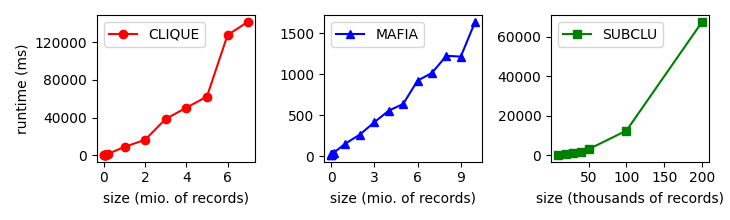
\includegraphics[scale=0.5]{figures/dataset_size_vs_runtime.png}
    \caption{Scalability with increasing data set size.}
    \label{fig:dataset_size_vs_runtime}
    \vspace*{-0.6cm}
\end{figure}

\subsubsection{Scalability with Data Dimensionality and Cluster Dimensionality}
Figure \ref{fig:data_dimensionality_vs_runtime} shows the scalability of the CLIQUE and MAFIA with increasing data set dimensionality. The data set contains 1mio. records with 3 clusters in 5 different subspaces, with 10\% noise. The dimensionality ranges from 10 to 100 dimensions. However, CLIQUE could only handle half of the dimensions, as the PC freezes due to the high memory consumption. To investigate this further, one could try to reduce the memory consumption by having a smaller amount of records in the data set. Nevertheless, from the experiment both seems to scale linearly with the data set dimensionality.
\begin{figure}[H]
    \vspace*{-0.6cm}
    \centering
    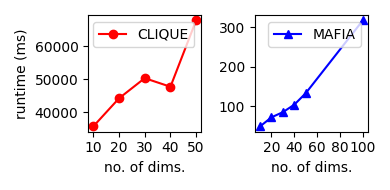
\includegraphics[scale=0.5]{figures/data_dimensionality_vs_runtime.png}
    \caption{Scalability with increasing data set dimensionality.}
    \label{fig:data_dimensionality_vs_runtime}
    \vspace*{-0.6cm}
\end{figure}

Figure \ref{fig:cluster_dimensionality_vs_runtime} shows the scalability of the CLIQUE and MAFIA with increasing cluster dimensionality. A 20-dimensional data set, containing 500k records with a single cluster was used, with the cluster embedded in an increasing number of dimensions, ranging from 10 to 100 dimensions. Additionally, 10\% of the records were noise. The data set is similar to the one used in \cite{mafia}. CLIQUE exhibits quadratic growth, while MAFIA shows primarily linear growth. However, MAFIA's runtime suddenly increases once the number of dimensions exceeds 15.
\begin{figure}[H]
    \vspace*{-0.6cm}
    \centering
    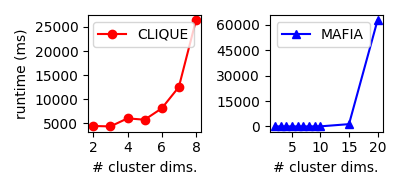
\includegraphics[scale=0.5]{figures/cluster_dimensionality_vs_runtime.png}
    \caption{Scalability with increasing cluster dimensionality.}
    \label{fig:cluster_dimensionality_vs_runtime}
    \vspace*{-0.6cm}
\end{figure}

An attempt was made to replicate the results for SUBCLU reported in \cite{subclu}, but the PC freezes due to the high memory consumption. In future work, it would be valuable to explore this further, possibly using a smaller number of records in the dataset.

% \subsection{Sensitive analysis for MAFIA}
% From \cite{mafia}, MAFIA should not be sensitive to the choice of $\alpha$. Therefore, a 20-dimensional data set with 1mio data points with 10\% noise were set to evaluate this. $\beta$ was fixed to 35\%, and $\alpha$ was ranging from 0.8 to 5.2 in step size of 0.4. The results can be seen in Figure \ref{fig:sensitivity_alpha}. From the results one could again draw the conclusion that MAFIA is not very sensitive to the $\alpha$ parameter. However, during evaluation of different types of data sets, many different values $\alpha$ was used to detect the right clusters. Also, different $\beta$ values as well as maximum number of windows was needed to be set properly to achieve meaningful results.
% \begin{figure}[H]
%     \vspace*{-0.6cm}
%     \centering
%     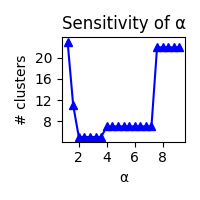
\includegraphics[scale=0.45]{figures/sensitivity_alpha.png}
%     \caption{Sensitivity of $\alpha$ for MAFIA.}
%     \label{fig:sensitivity_alpha}
%     \vspace*{-0.6cm}
% \end{figure}

\subsubsection{Clustering Accuracy}
Several synthetic datasets were generated to evaluate the clustering accuracy of the algorithms. It is important to note that the results were based on visual inspection of the clusters, as the external metrics available in ELKI are not well-suited for subspace clustering \cite{e4sc}. Although an attemt was made to implement the subspace clustering evaluation metric \textit{E4SC} and the \textit{clustering error} (CE) \cite{e4sc}, the implementation was unsuccessful.

The first dataset was a 2-dimensional set with a single skewed-plus-sign shaped cluster and 10\% noise. Results similar to those reported in \cite{mafia} were achieved. MAFIA successfully identified a single cluster that accurately captured the cluster's boundaries. In contrast, CLIQUE was unable to report a single cluster that correctly detected the borders. However, MAFIA's accuracy comes at a cost, as it also identifies many lower-dimensional clusters.

% The results can be seen in Figure \ref{fig:accuracy_plus}, where only the best cluster found by MAFIA is illustrated. The effect of adaptive grid sizes, clearly shows that MAFIA is more flexible than CLIQUE in such cases.
% \begin{figure}[H]
%     \vspace*{-0.6cm}
%     \centering
%     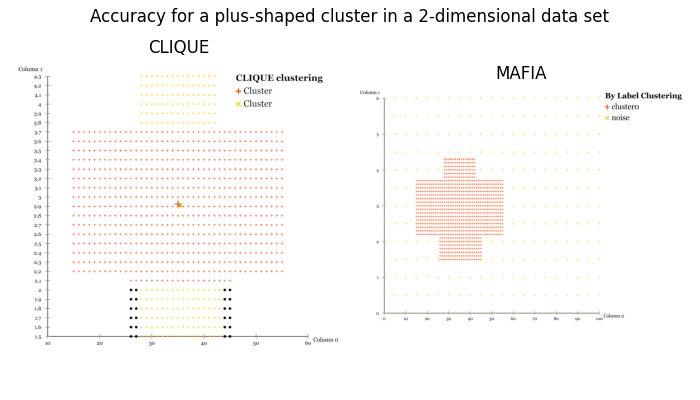
\includegraphics[scale=0.35]{figures/accuracy_plus.png}
%     \caption{A single plus-shaped cluster.}
%     \label{fig:accuracy_plus}
%     \vspace*{-0.6cm}
% \end{figure}

The second dataset was a 10-dimensional set containing 2 clusters embedded in a different 4 dimensional subspace, with 10\% noise. This dataset was similar to the one used in \cite{mafia}. The results are shown in Figure \ref{fig:accuracy_2clusters}. MAFIA successfully detected both clusters without identifying any additional lower-dimensional clusters. In contrast, CLIQUE reports some overlapping clusters and misclassified some noise records as clusters. SUBCLU also detected the two clusters but, like CLIQUE, it identified many lower-dimensional clusters and classified noise records as clusters.
\begin{figure}[H]
    \vspace*{-0.6cm}
    \hspace*{-0.6cm}
    \centering
    \subfloat[][CLIQUE]{%
        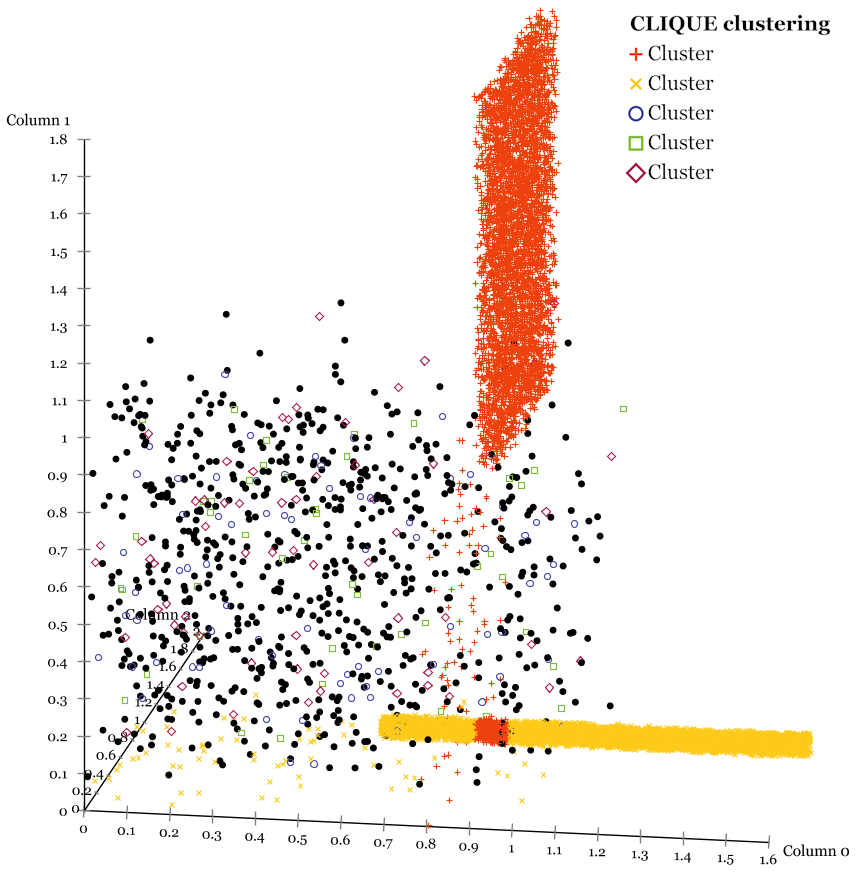
\includegraphics[width=0.35\textwidth]{figures/accuracy_2clusters/clique.png}\label{fig:accuracy_2clusters_clique}}~~
    \subfloat[][MAFIA]{%
        \includegraphics[width=0.35\textwidth]{figures/accuracy_2clusters/MAFIA.png}\label{fig:accuracy_2clusters_mafia}}~~
    \subfloat[][SUBCLU]{%
        \includegraphics[width=0.35\textwidth]{figures/accuracy_2clusters/SUBCLU.png}\label{fig:accuracy_2clusters_subclu}}
    \caption{Two clusters in 4 different subspaces.}
    \label{fig:accuracy_2clusters}
    \vspace*{-0.6cm}
\end{figure}

The third dataset were a 2-dimensional set containing a single cluster formed as a Bezier curve, with 10\% noise. As expected, SUBCLU outperformed the other two, as shoen in Figure \ref{fig:accuracy_bezier}. MAFIA and CLIQUE only partially detected the cluster and misclassified additional clusters and noise records.
\begin{figure}[H]
    \vspace*{-0.6cm}
    \hspace*{-0.6cm}
    \centering
    \subfloat[][CLIQUE]{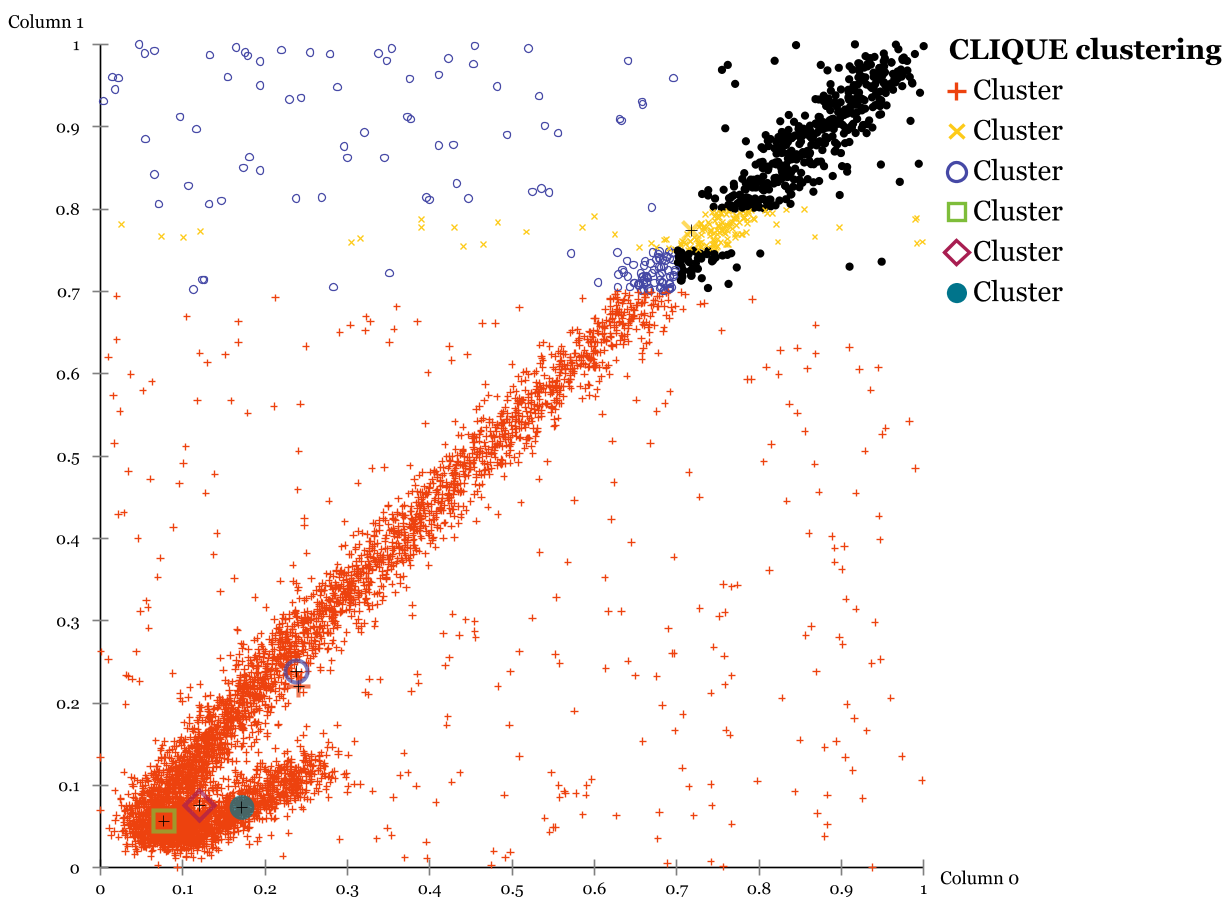
\includegraphics[width=0.35\textwidth]{figures/accuracy_bezier/clique.png}\label{fig:accuracy_bezier_clique}}~~
    \subfloat[][MAFIA]{\includegraphics[width=0.35\textwidth]{figures/accuracy_bezier/MAFIA.png}\label{fig:accuracy_bezier_mafia}}~~
    \subfloat[][SUBCLU]{\includegraphics[width=0.35\textwidth]{figures/accuracy_bezier/SUBCLU.png}\label{fig:accuracy_bezier_subclu}}
    \caption{A single bezier-shaped cluster.}
    \label{fig:accuracy_bezier}
\end{figure}

\subsubsection{Real Data Sets}
Two real-world data sets are used to evaluate the algorithms in a more realistic setting. Small data sets were selected for both performance and visualization reasons. Both data sets were normalized to the range [0, 1].

The first data set is the well-known \textit{Iris} data set \cite{iris}, which contains 150 records of 3 different iris species with 4 features. All three algorithms successfully generated clusters, however, the overall clustering quality was suboptimal.
% \begin{figure}[H]
%     \vspace*{-0.6cm}
%     \centering
%     \subfloat[][Original]{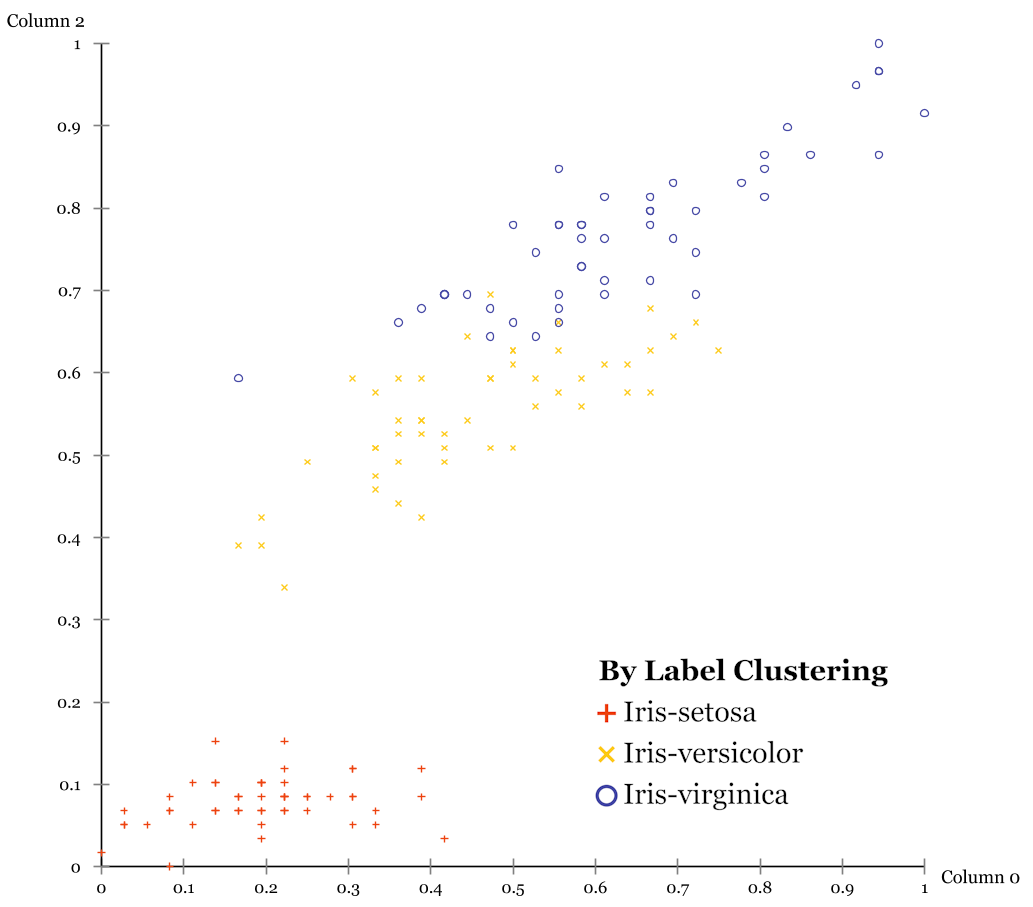
\includegraphics[width=0.3\textwidth]{figures/real_world_iris/orig.png}\label{fig:real_world_iris_orig}}~~~~
%     \subfloat[][CLIQUE]{\includegraphics[width=0.3\textwidth]{figures/real_world_iris/CLIQUE.png}\label{fig:real_world_iris_clique}}\\
%     \subfloat[][MAFIA]{\includegraphics[width=0.3\textwidth]{figures/real_world_iris/MAFIA.png}\label{fig:real_world_iris_mafia}}~~~~
%     \subfloat[][SUBCLU]{\includegraphics[width=0.3\textwidth]{figures/real_world_iris/SUBCLU.png}\label{fig:real_world_iris_subclu}}
%     \caption{Iris data set.}
%     \label{fig:real_world_iris}
%     \vspace*{-0.6cm}
% \end{figure}

The second data set is the \textit{Date Fruit} data set \cite{date-fruit}, consiting of 898 records of 7 different types of date fruit with 34 features. Only SUBCLU were able to produce clusters somewhat close to the true clusters but also finds many lower-dimensional clusters and small clusters. CLIQUE and MAFIA either produced too many clusters or close to one single cluster.
% \begin{figure}[H]
%     \vspace*{-0.6cm}
%     \centering
%     \subfloat[][Original]{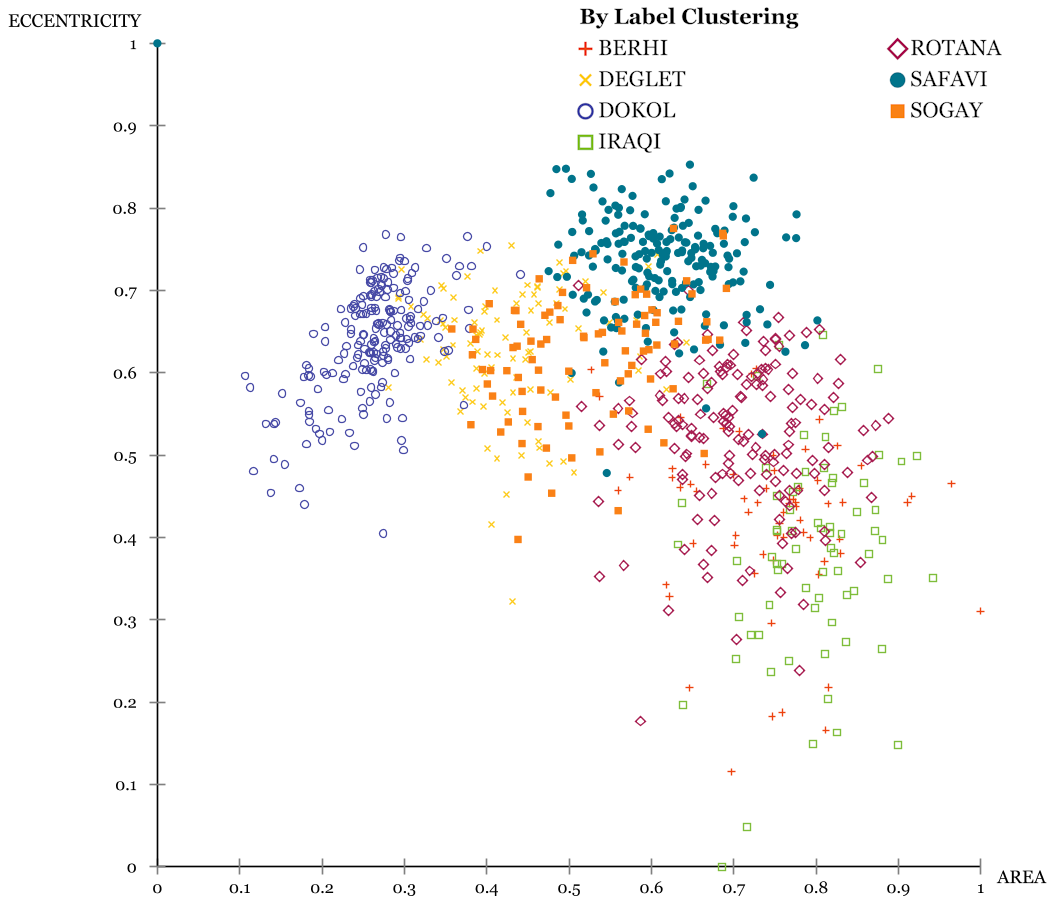
\includegraphics[width=0.3\textwidth]{figures/real_world_date_fruit/orig.png}\label{fig:real_world_date_fruit_orig}}~~~~
%     \subfloat[][SUBCLU]{\includegraphics[width=0.3\textwidth]{figures/real_world_date_fruit/SUBCLU.png}\label{fig:real_world_date_fruit_subclu}}
%     \caption{Date Fruit data set.}
%     \label{fig:real_world_date_fruit}
%     \vspace*{-0.6cm}
% \end{figure}